\begin{appendices}

	
\section {Appendix: Regulatory compliance}

% It must be noted that since the project is a research project, most of the regulations here exposed may not be needed. 
% Nevertheless, they must be taken into account in the case that the system is commercialized.

	% \paragraph{ISO}\mbox{}\\

	% The International Organization for Standardization is an international organism that settles international standards. 
	% It has several joint committees with the International Electrotechnical Commission (IEC). 
	% They develop standards in different technical fields such as the electrical, electronic or IT fields. 
	% \\

	% The Information Technology (IT) term is related to the use of computers and telecommunications to interchange, store and manipulate data.  
	% It is a broad field in which the present project may be included.
	% The Joint Technical Committee devoted to this subject is the ISO/IEC JTC 1. 
	% Its main mission is develop, maintain, promote and facilitate IT standards regarding different areas such as the following : 
	% \begin{itemize}
	% 	\item{Design and development of systems and tools}
	% 	\item{Define performance and quality standards}
	% 	\item{Security, interoperability and portability of IT systems and products}
	% 	\item{Unified tools and environments as well as harmonized IT vocabulary}
	% \end{itemize}

	% This Committee has recently included the regulations regarding assistive tecnology (AT) \cite{japan1}\cite{japan2}.
	% %--> http://en.wikipedia.org/wiki/ISO/IEC_JTC_1 [IT projects] 


	% \paragraph{Software regulations}\mbox{}\\
		% This section is centered on the ones related to Open Source systems, since the software developed in this thesis is Open  
	The present section covers the regulatory compliance that affects directly to the system presented. 
	% There are different regulations regarding software. 
	% Since the project is Open Source, this section focus on presenting the regulations of this type of systems. \\
	Nowadays, the author of the software has the right of sharing it using a contract. 
	In it he determines which of the author rights he is going to yield and under what conditions. 
	This type of contract is called a software license. 
	% This project uses a number of third-party libraries that have their own license. 
	Sections \ref{ocular} to \ref{pcl} show the details of the licenses of this thesis and the third-party libraries being used. 

	\subsection{OpenCV}
	The Open Source Computer Vision library is released under a BSD license. 
	Hence it is free for both academic and commercial use. 
	Nevertheless, there are certain algorithms implemented whose license is different from the whole library. 
	The SIFT or SURF descriptors are two examples of this fact: they have a software patent. 
	This legal figure allows the use of the algorithms for investigation purposes, but imposes the payment of a fee for commercial uses. 
	Since OCULAR is intended to be an Open Source system, neither of these algorithms are used.
	Instead, the ORB algorithm is utilized in the system.% as the descriptor extractor of the system. 
	ORB has no patent and hence can be incorporated in software designed for both commercial and research uses. 

	\subsection{PCL}
	\label{pcl}
	The Point Cloud Library has as well a BSD license. 
	It is then free for commercial and research use. 
	Further information about the library and its license may be found in this \href{http://pointclouds.org}{\color{blue} {webpage}} \footnote{http://pointclouds.org}. 


	\subsection{ROS}
	All ROS core code is distributed under a BSD license, more specifically a BSD 3-Clause license. 
	It is very similar to the OCULAR license, the redistribution is permitted under certain conditions. 
	More information may be found in this \href{http://opensource.org/licenses/BSD-3-Clause}{\color{blue} {webpage}}\footnote{http://opensource.org/licenses/BSD-3-Clause}. 
	The different ROS packages that are used in this thesis (openni\_camera, openni\_launch and pi\_tracker) are distributed under a BSD license, according to their web pages ( \href{http://wiki.ros.org/openni_camera}{openni\_camera}\footnote{http://wiki.ros.org/openni_camera}, \href{http://wiki.ros.org/openni_launch}{openni\_launch}\footnote{http://wiki.ros.org/openni_launch}, \href{http://wiki.ros.org/pi_tracker}{pi\_tracker} \footnote{http://wiki.ros.org/pi\_tracker}).


	\subsection{OCULAR}
	\label{ocular}
	The license of this system must be coherent with the ones of the third-party libraries it uses.
	In fact, Open Source packages and libraries were selected to ensure that the whole system could be free for commercial and research use. 
	This is the reason why this project is being distributed with a MIT License (MIT). 
	The MIT license may be found in this  \href{https://raw.githubusercontent.com/irenesanznieto/ocular/master/LICENSE.md}{\color{blue}\underline {link}}\footnote{https://raw.githubusercontent.com/irenesanznieto/ocular/master/LICENSE.md}, and states the following: \\

	"Copyright (c) 2014 Irene Sanz Nieto

Permission is hereby granted, free of charge, to any person obtaining a copy of this software and associated documentation files (the "Software"), to deal in the Software without restriction, including without limitation the rights to use, copy, modify, merge, publish, distribute, sublicense, and/or sell copies of the Software, and to permit persons to whom the Software is furnished to do so, subject to the following conditions:

The above copyright notice and this permission notice shall be included in all copies or substantial portions of the Software.

The software is provided "as is", without warranty of any kind, express or implied, including but not limited to the warranties of merchantability, fitness for a particular purpose and noninfringement. In no event shall the authors or copyright holders be liable for any claim, damages or other liability, whether in an action of contract, tort or otherwise, arising from, out of or in connection with the software or the use or other dealings in the software."
\\

	The last paragraph is published in uppercase letters, but it was converted to lowercase to avoid a disturbance in the structure of the thesis. 	
	The license claims that software is available for redistribution and use, but no warranty is provided with it. 
	The different algorithms and third-party packages were selected taking into account that their licenses must be compatible with the one being provided by this system. 
	In the next sections the licenses under which the different packages are distributed are presented. 
	\\

	Apart from the licensing of the software, it was taken into account in the development of the system that this project needs to store the information learned to be able to use it in later sessions. % involves taking personal information to construct a dataset with which recognize different objects. 
	In order to observe the data protection Spanish law (Ley Orgánica 15/1999, de 13 de diciembre, de Protección de Datos de Carácter Personal), the stored data does not contain any personal information. 
	Instead of storing, for example, an image of the user, the information retrieved is a matrix of numbers containing the descriptors extracted from the objects. 
	This ensures that the system could be used in commercial software or that further investigations could be performed accordingly with the law. 





	% \paragraph{Data protection} \mbox{}
	\\

	% Since this project implements a proof of concept, the experiments performed with it were done by the author. 
	

	% This law "warrants and protects the personal data treatment, the public liberties and the fundamental rights of the persons, specially their honor and personal and familiar intimacy".
	% It is applicable to all data stored in a physical support. 
% 	Privacidad y confidencialidad: cualquier investigación que contenga datos de caracter personal tiene que cumplir los preceptos de la legislación de protección de datos. En España la norma que regula estos aspectos es la Ley Orgánica 15/1999, de 13 de diciembre, de Protección de Datos de Carácter Personal, cuayo objeto es 'garantizar y proteger en lo que concierne al tratamiento de los datos personales, las libertades públicas y los derechos fundamentales de las personas físicas, y especialmente de su honor e intimidad personal y familiar”.
% La ley es de aplicación a los datos de carácter personal registrados en cualquier soporte físico. El tratamiento de los datos cubre las actividades de recolección, registro, almacenamiento, recuperación, consulta, uso y diseminación. Para garantizar el derecho a la protección de datos, es necesario informar a las personas implicadas y solicitar su consentimiento para el tratamiento de sus datos. 

	\chapter{Software requirements specification}
			\includepdf[pages={-}]{backmatter/requisites/requisites.pdf}
			%\documentclass{article}
\usepackage[utf8]{inputenc}
\usepackage{amsmath}
\usepackage{graphicx}
\usepackage{listings}
\usepackage[top=1.55cm, bottom=2.29cm, left=1.6cm, right=1.47cm]{geometry}
% This is for the fancy title in each page
\usepackage{fancyhdr}
\lhead{}
\chead{}
\rhead{First Session: Combinational Design}
\pagestyle{fancy}

\usepackage{enumitem}


\makeatletter
\def\threedigits#1{\expandafter\@threedigits\csname c@#1\endcsname}
\def\@threedigits#1{%
  \ifnum#1<100 0\fi
  \ifnum#1<10 0\fi
  \number#1}
\makeatother
\AddEnumerateCounter{\threedigits}{\@threedigits}{100}


%\setenumerate[1]{}


\begin{document}

%%%% FRONTPAGE %%%%%%%%%%%%%%%%%%%%%%%%%%%%%%%%%%%%%%%%%%%%%%%%%%%%%%%%%%%
\begin{titlepage}

\begin{center}
%
\includegraphics[width=0.25\textwidth]{./uc3m.jpg}\\[2cm]
\textsc{\huge Bachelor's Thesis:\\[0.5cm]In-hand object detection and tracking using\\[0.5cm]2D and 3D
information }\\[4cm]


% Title
{\Huge\bfseries{Software Requirements Specification}\\[2cm]}

\Large{Version 0.2}
\\[11cm]


% Author and supervisor
\begin{minipage}{0.55\textwidth}
\begin{flushleft} \large
\emph{Author:}\\
Irene Sanz Nieto\\
\end{flushleft}
\end{minipage}
\begin{minipage}{0.4\textwidth}
\begin{flushright} \large
\emph{Supervisor:}\\
Victor González Pacheco\end{flushright}\end{minipage}\vfill

% Bottom of the page
{\large \today}

\end{center}
\end{titlepage}

%
\newpage
%
%%%%%%Table of contents%%%%%%%%%%%%%%%%%%%%%%%%%%%%%%
%%%%%%%%%%%%%%%%%%%%%%%%%%%%%%%%%%%%%%%%%%%%%%%%%%%%%
\tableofcontents
\newpage


%%%%%%Document%%%%%%%%%%%%%%%%%%%%%%%%%%%%%%%%%%
%%%%%%%%%%%%%%%%%%%%%%%%%%%%%%%%%%%%%%%%%%%%%%%%%%%%%
\section{Introduction}
\hspace{0.5cm}The project consists on an in-hand object learning and recognition software. 
%
\includegraphics[width=0.25\textwidth]{./uc3m.jpg}\\[2cm]
\subsection{Nodes}

\subsubsection{Event Handler Node}
	This node will identify the different user's gestures and act accordingly using a State Machine structure. 
	\begin{center}
		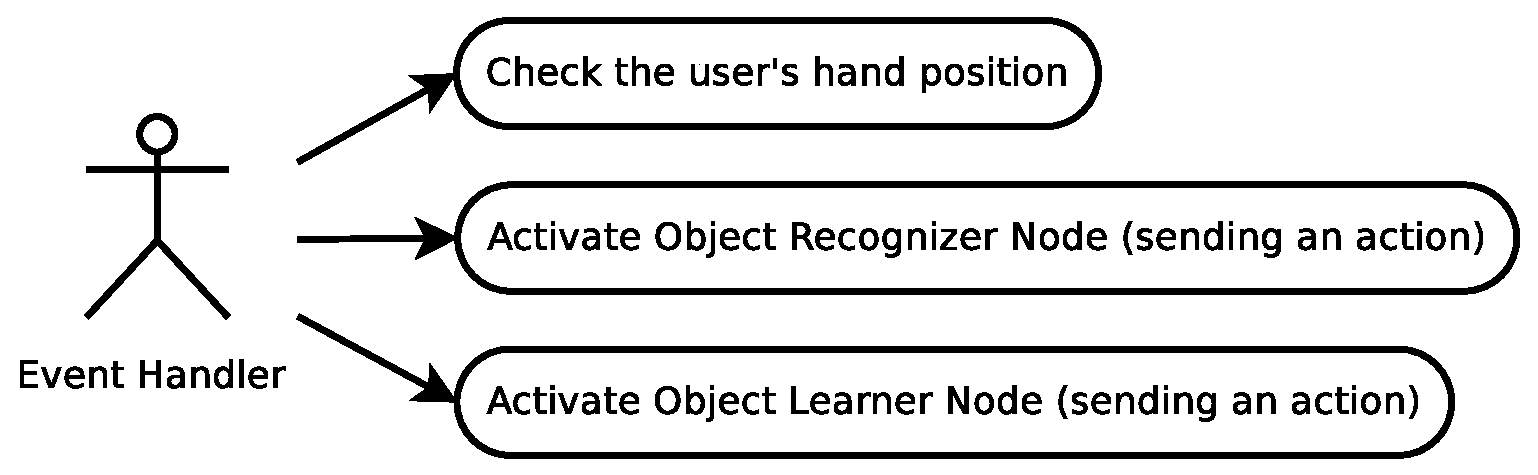
\includegraphics[scale=0.4]{../diagrams/images/uc_event_handler.eps}
	\end{center}
	
\subsubsection{Display Node}
This node shows the output of the program. There is a window in which different information will be shown. 
	\begin{center}
		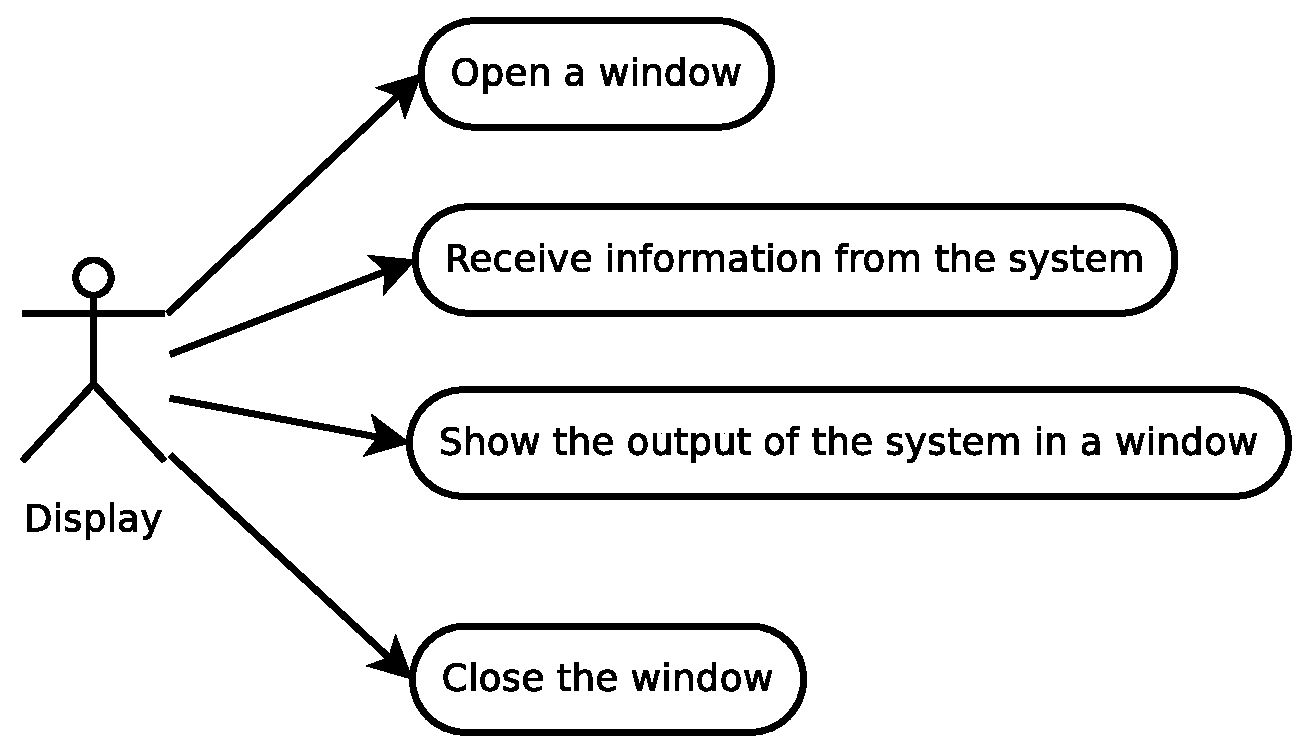
\includegraphics[scale=0.4]{../diagrams/images/uc_display.eps}
	\end{center}
	
\subsubsection{Object Learner Node}

\hspace{0.5cm}This node learns 2D and 3D features extracted from the handheld object using a RGB-D sensor.   

The sequence of the object learning is the following:
\\
First, 3D and 2D descriptors are extracted and written to a file. Then, two algorithms are trained (one for 2D and the other for the 3D template). The parameters of each trained algorithm are stored in a file. There will be hence one file per learned object and one file per algorithm.
\\

The learning of the objects is done in-hand. The training starts when the user extends the hand in front of the body, showing the new object to the RGB-D sensor. Then, the user rotates the object to allow the software to extract the features of different views to obtain a more robust model of the object. This way of learning new objects will allow a more intuitive interaction human-robot. When the user returns the arm to a position which is closer to the body, the algorithm starts learning the new object and after the learning, it comes back to the recognizing mode, which is the default. 

\begin{center}

		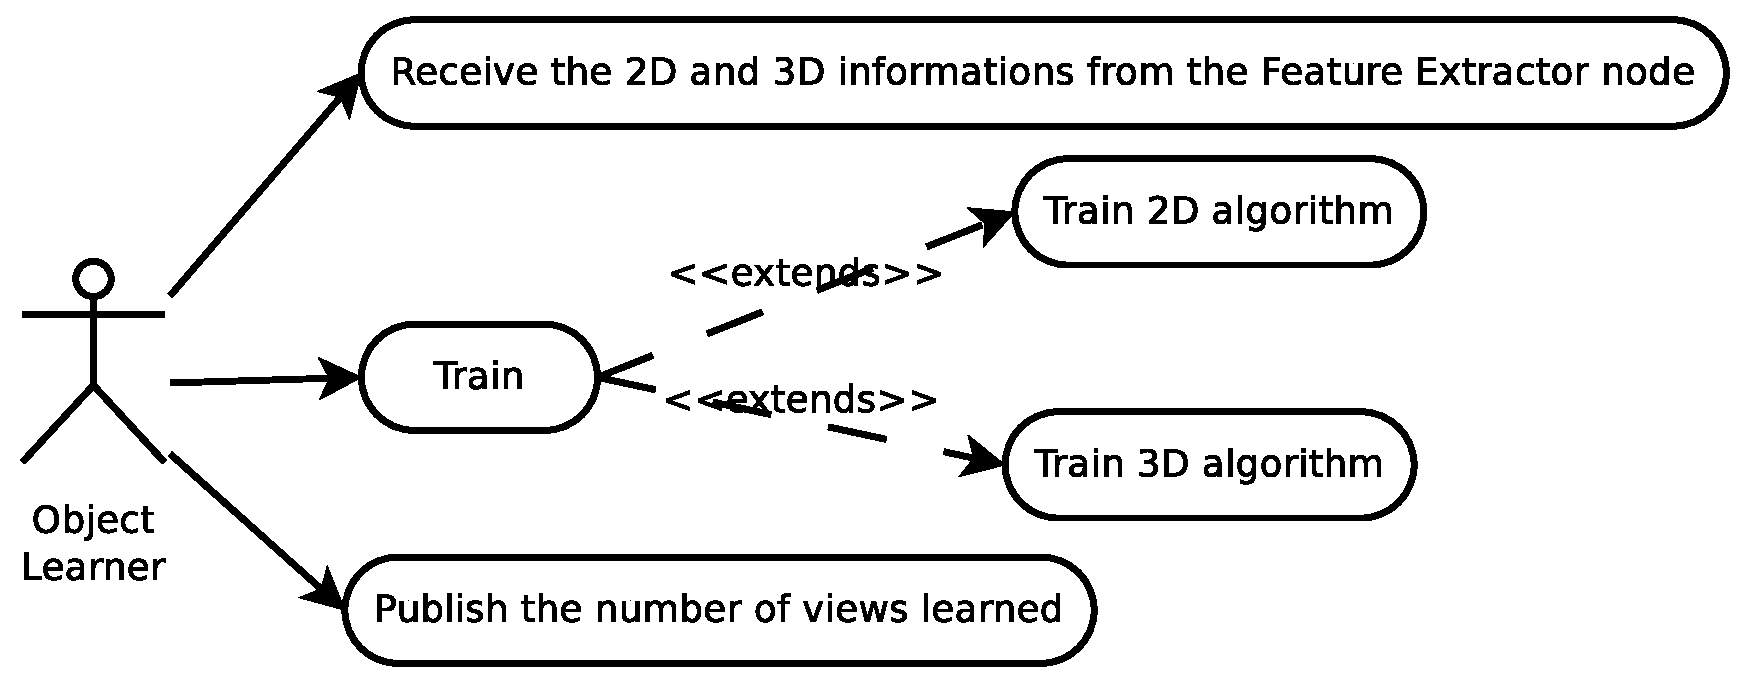
\includegraphics[scale=0.4]{../diagrams/images/uc_learner.eps}
	\end{center}

\subsubsection{Object Recognizer Node} 
\hspace{0.5cm}This node will track the user's hands and recognize the held objects. 

There are two different algorithms, one trained with the 2D data and the other one trained with the 3D data. More information about those algorithms may be found in the Functional Requirements section. 
\\
The steps done by this node are the following: 
First, as in the Learning Mode, 2D and 3D descriptors will be extracted. Then, the algorithms will compare that information with the learned one. 
The output of each algorithm will be a percentage of similarity between the dataset and the new object. 
\\
The 3D information is more reliable than the 2D. The latter is subjected to inaccuracies due to illumination or view angle that affects the descriptors extracted and hence the object recognition.
\\
Due to this fact, weights for the output of each algorithm will be given. Those give a higher importance to the 3D descriptors since they are more robust. 
\\
The object that is finally published in a topic will be the one with a higher percentage of similarity. 

\begin{center}
	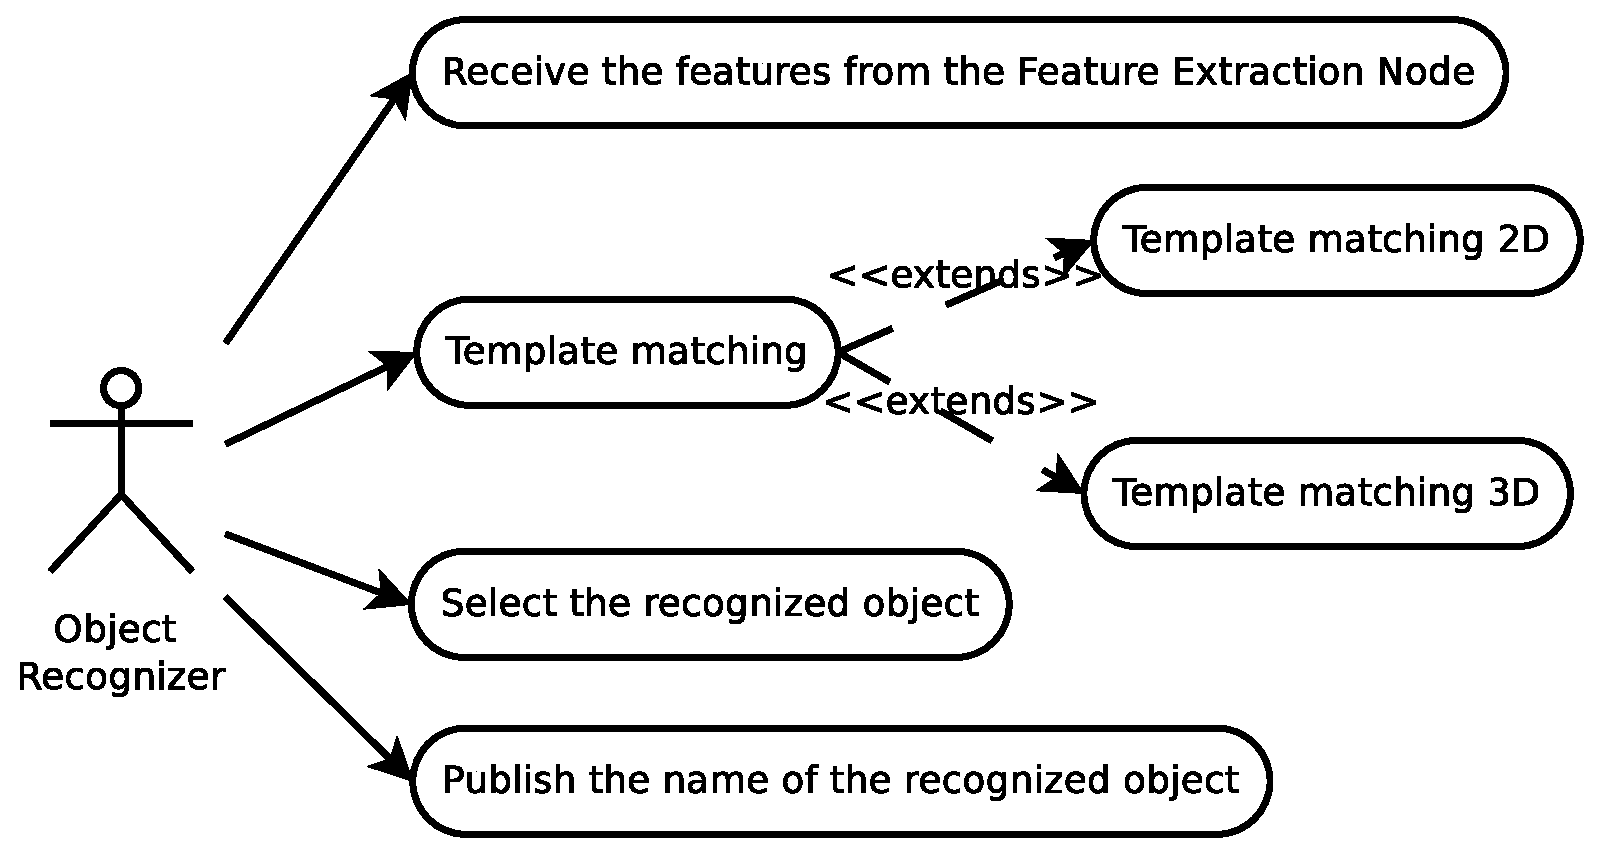
\includegraphics[scale=0.4]{../diagrams/images/uc_recognizer.eps}
\end{center}

\subsubsection{Converter Node}

This node will convert the messages from other ROS packages to the internal message format used within the code. 

\begin{center}
	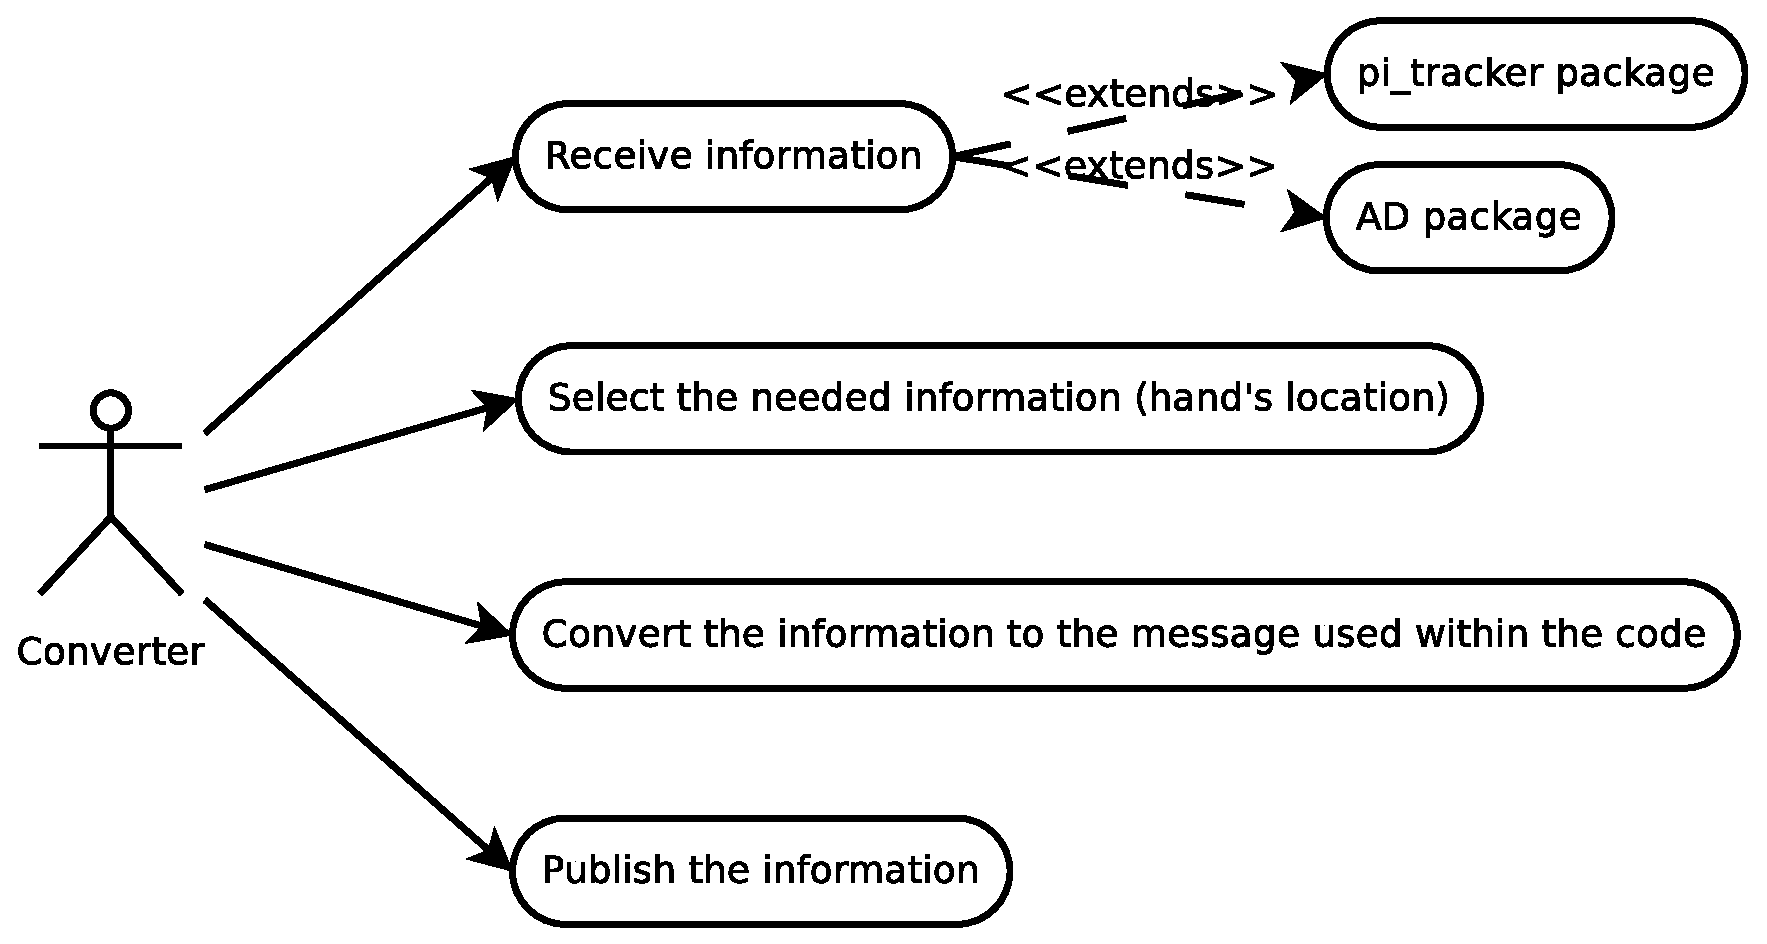
\includegraphics[scale=0.4]{../diagrams/images/uc_converter.eps}
\end{center}
	
\subsubsection{ROI Segmenter Node}
This node will segment the ROI (Region Of Interest) both in 2D and 3D.

\begin{center}
	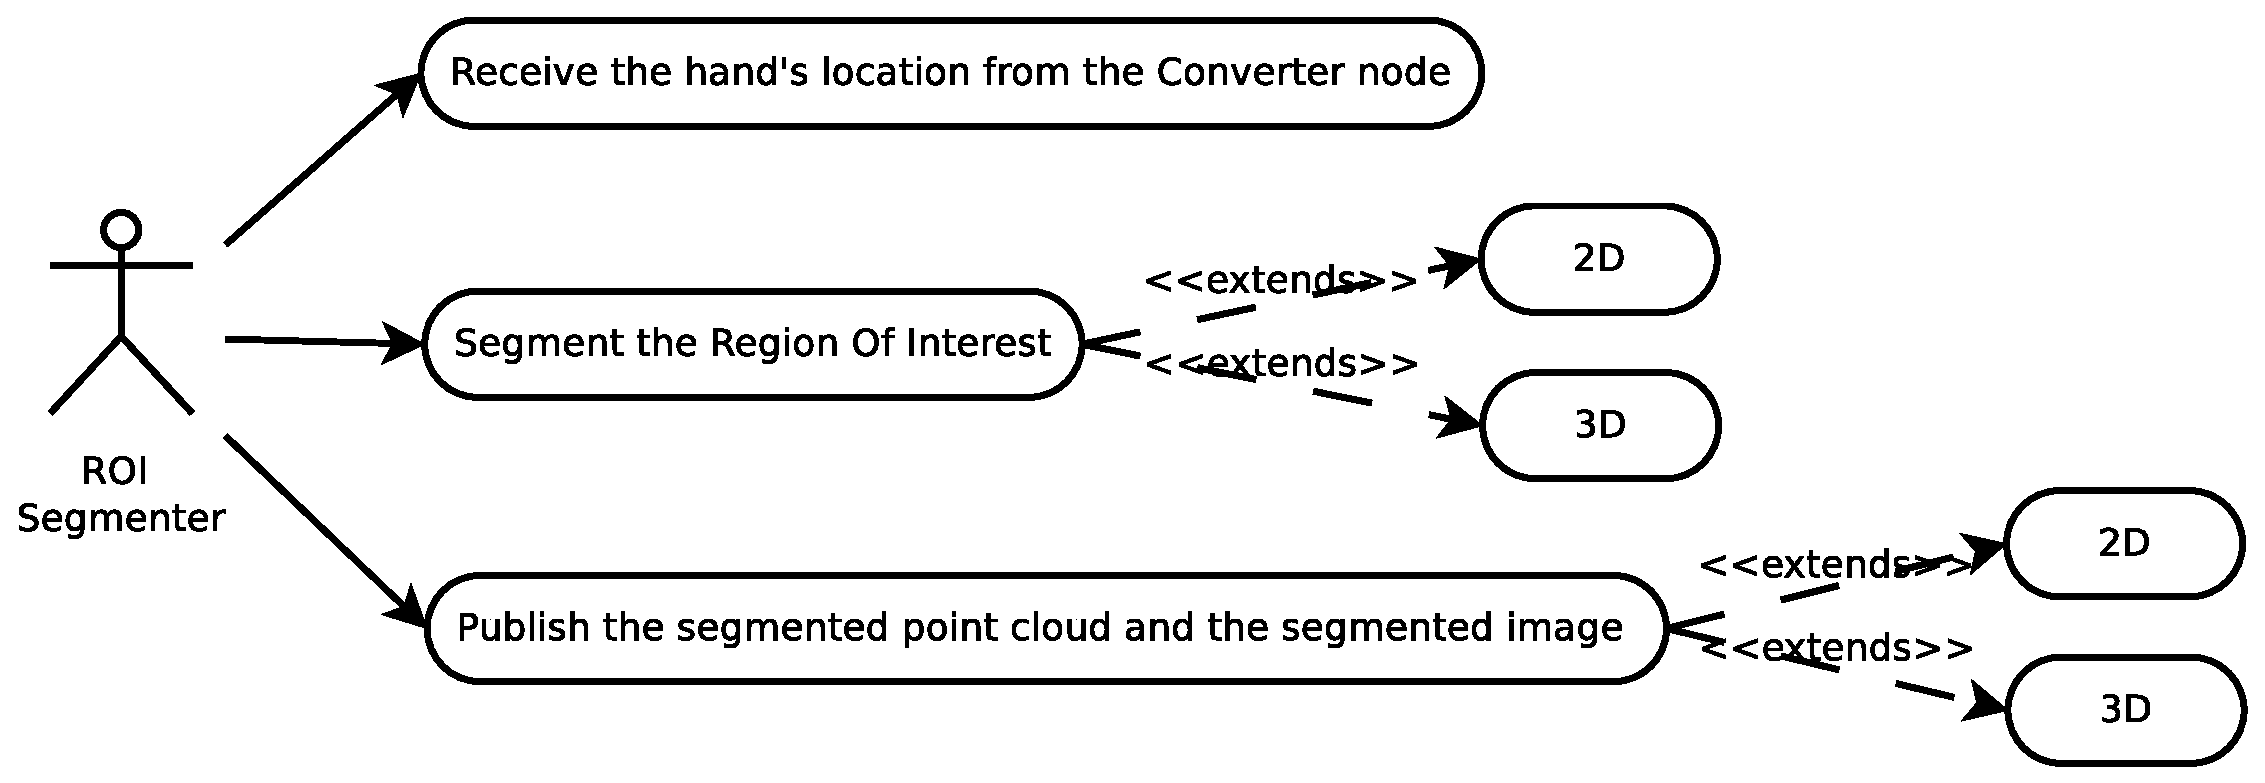
\includegraphics[scale=0.4]{../diagrams/images/uc_roi_segmenter.eps}
\end{center}

\subsubsection{Feature Extractor Node}
This node will extract both 2D and 3D features and publish them. 

\begin{center}
	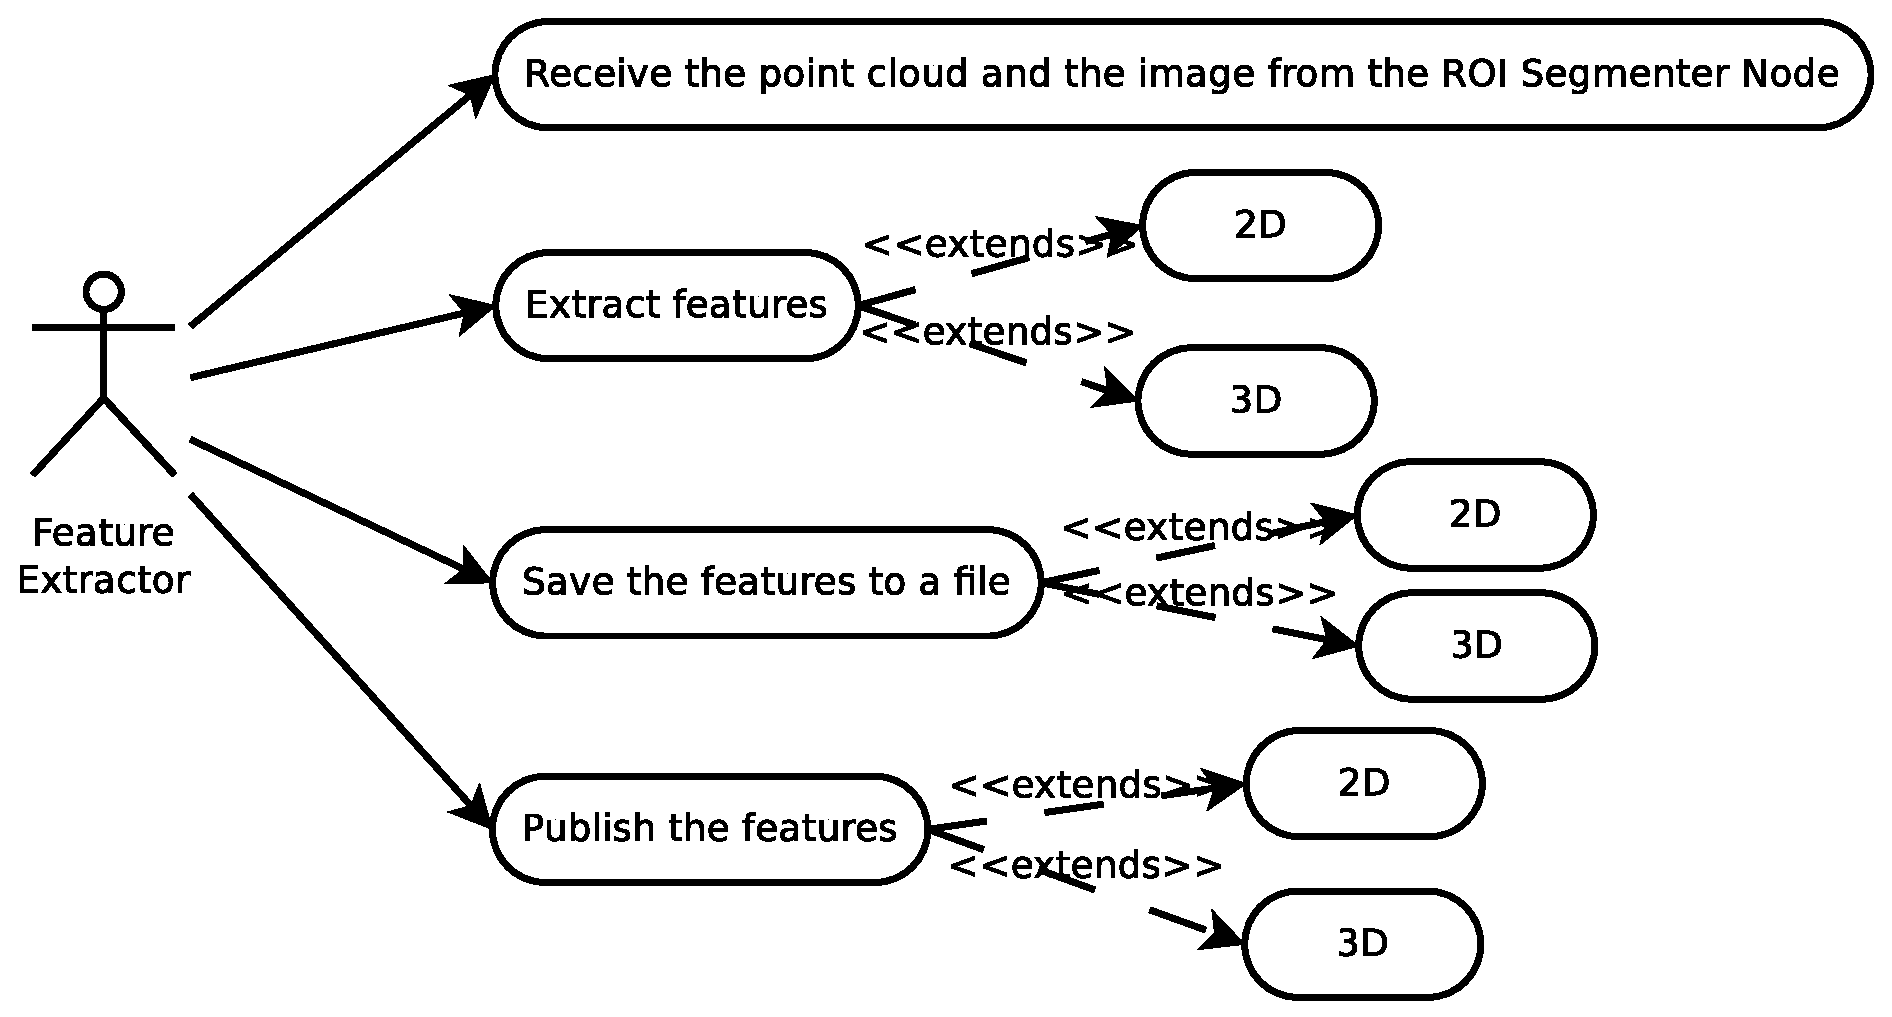
\includegraphics[scale=0.4]{../diagrams/images/uc_feature_extractor.eps}
\end{center}


\subsubsection{Data Parser Node}
This node will store the 2D and 3D features of each template of the same object in one file. 
\begin{center}
	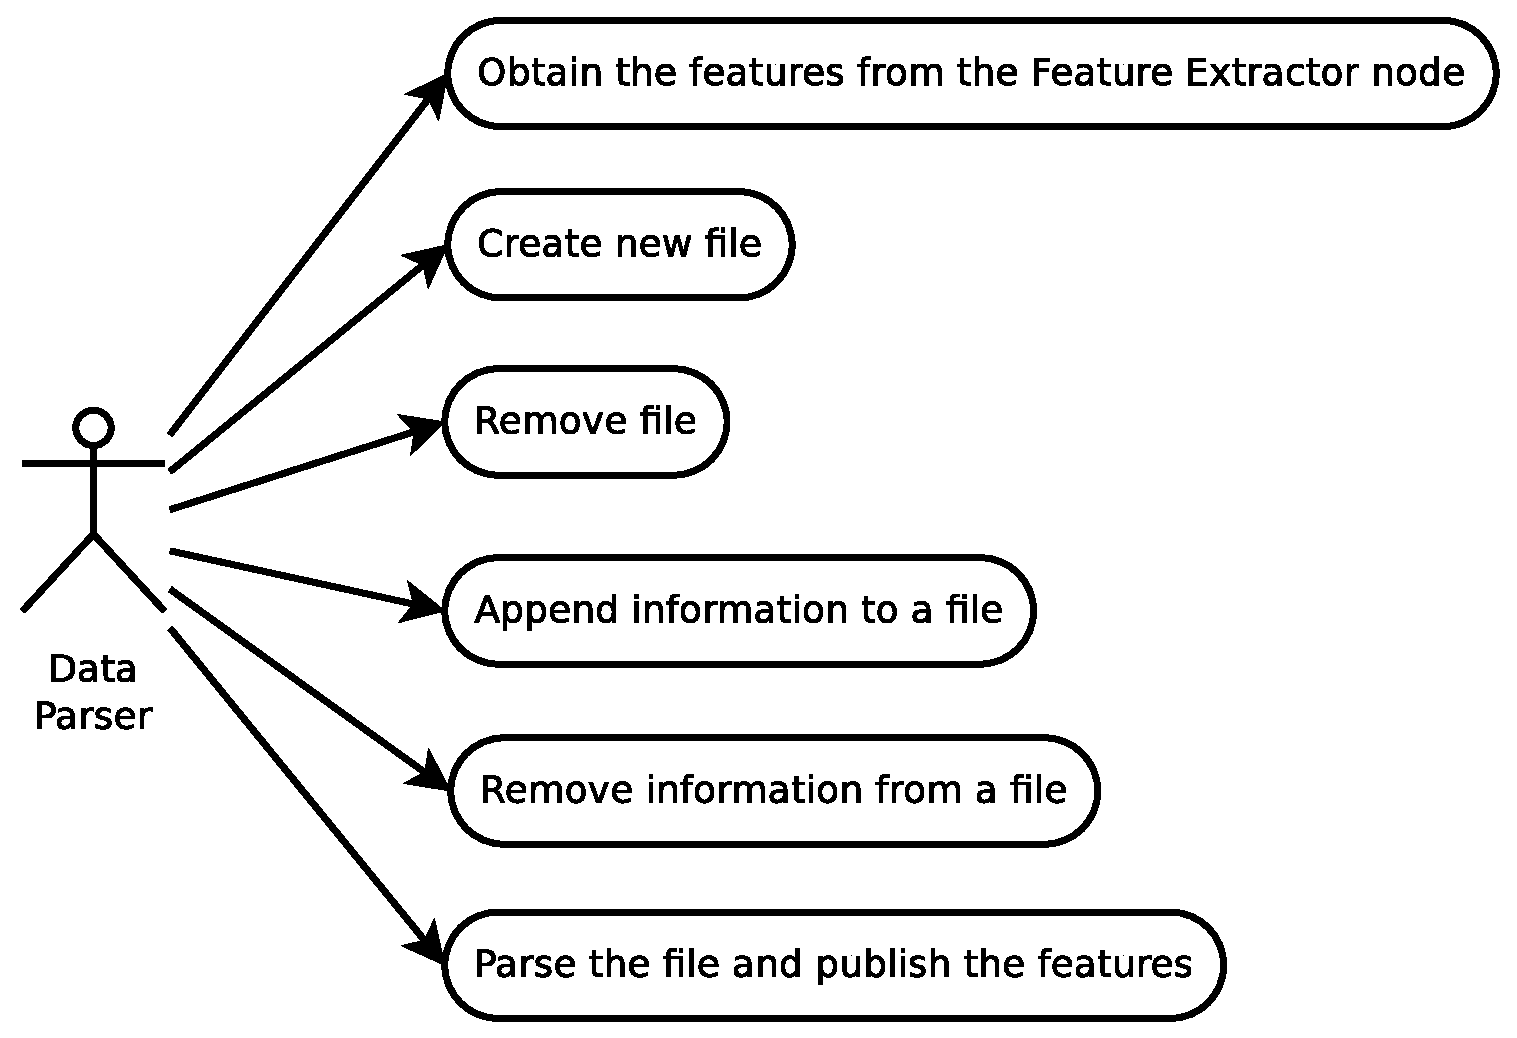
\includegraphics[scale=0.4]{../diagrams/images/uc_data_parser.eps}
\end{center}


\subsection{Third Party Packages}
\hspace{0.5cm}Initially only one third party ROS package will be used, to track the hand's position: pi\_ tracker. This software publishes the hand's position and there will a node in the proposed software (Conversion Node, whose requirements are specified in the next section) that converts the information returned by pi\_ tracker to the custom message used in the rest of the code.  

\subsection{Node Interaction}
%In the following diagram it can be seen the interaction and the information exchanged between nodes.
%\subsubsection{Use Case Diagram}
%\begin{center}
%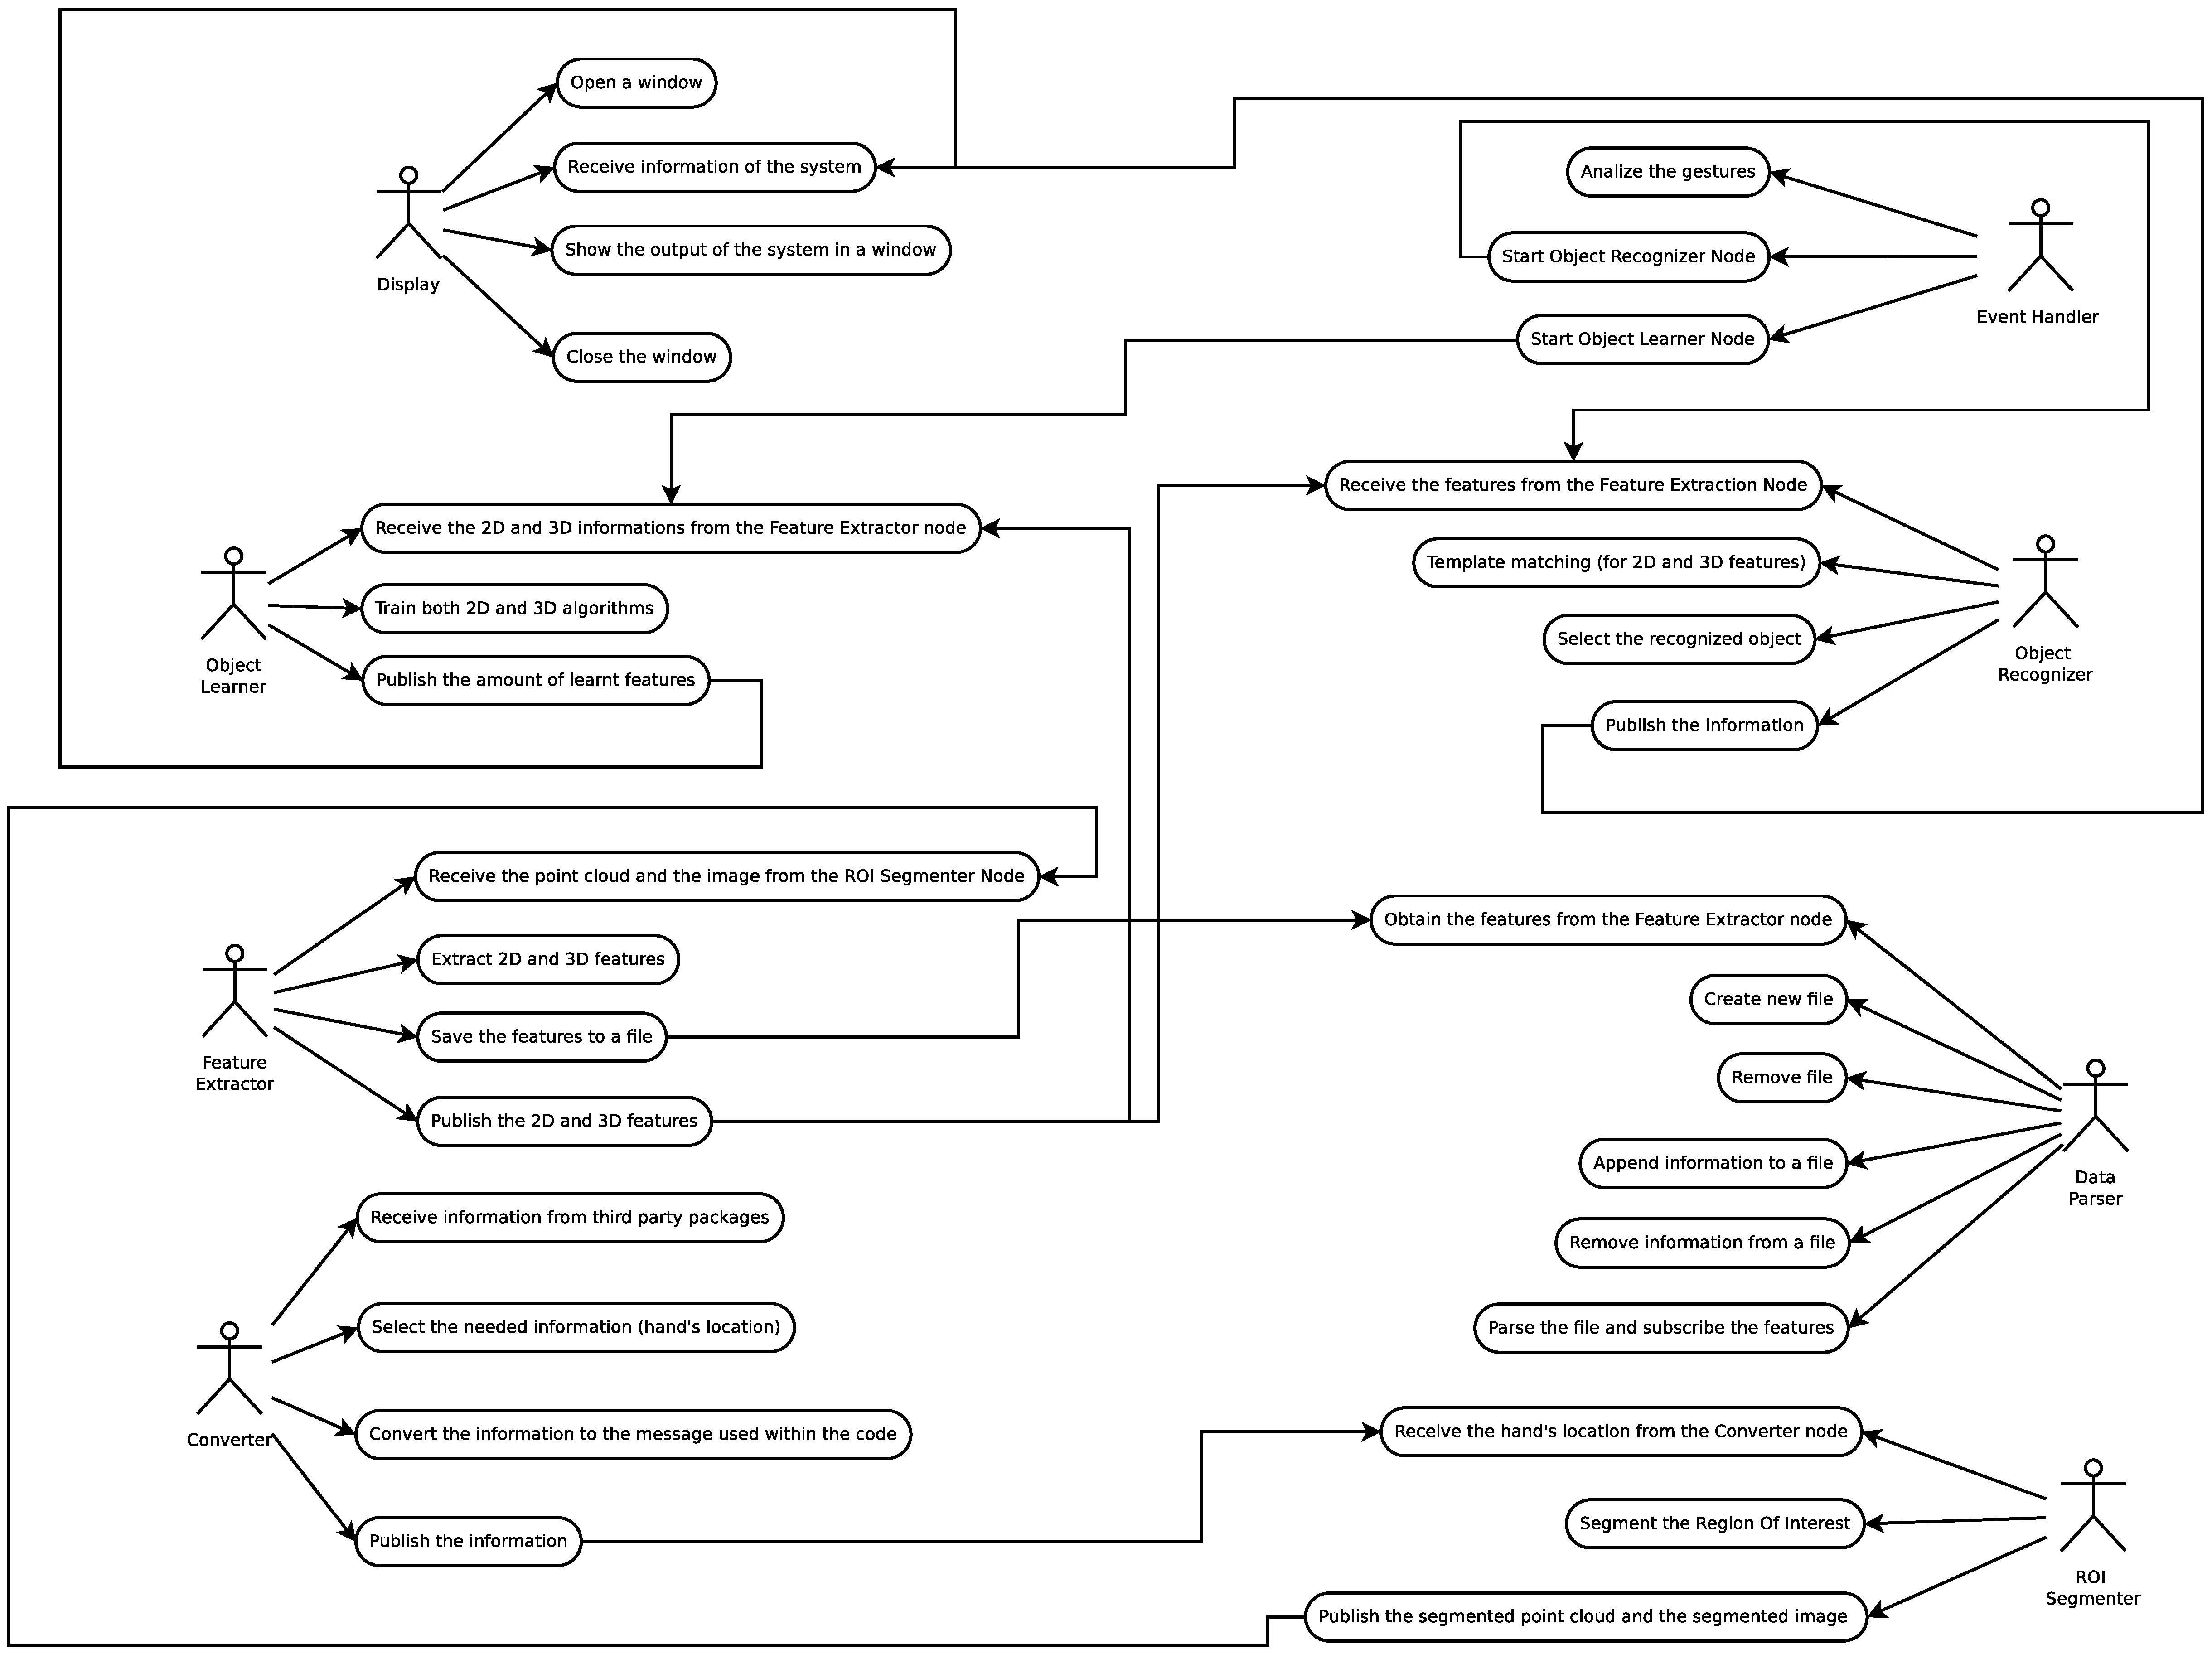
\includegraphics[scale=0.3]{../diagrams/images/use_case.eps}
%\end{center}

\subsubsection{Sequence Diagram}
In the following diagram can be seen the interaction between nodes. 
\begin{center}
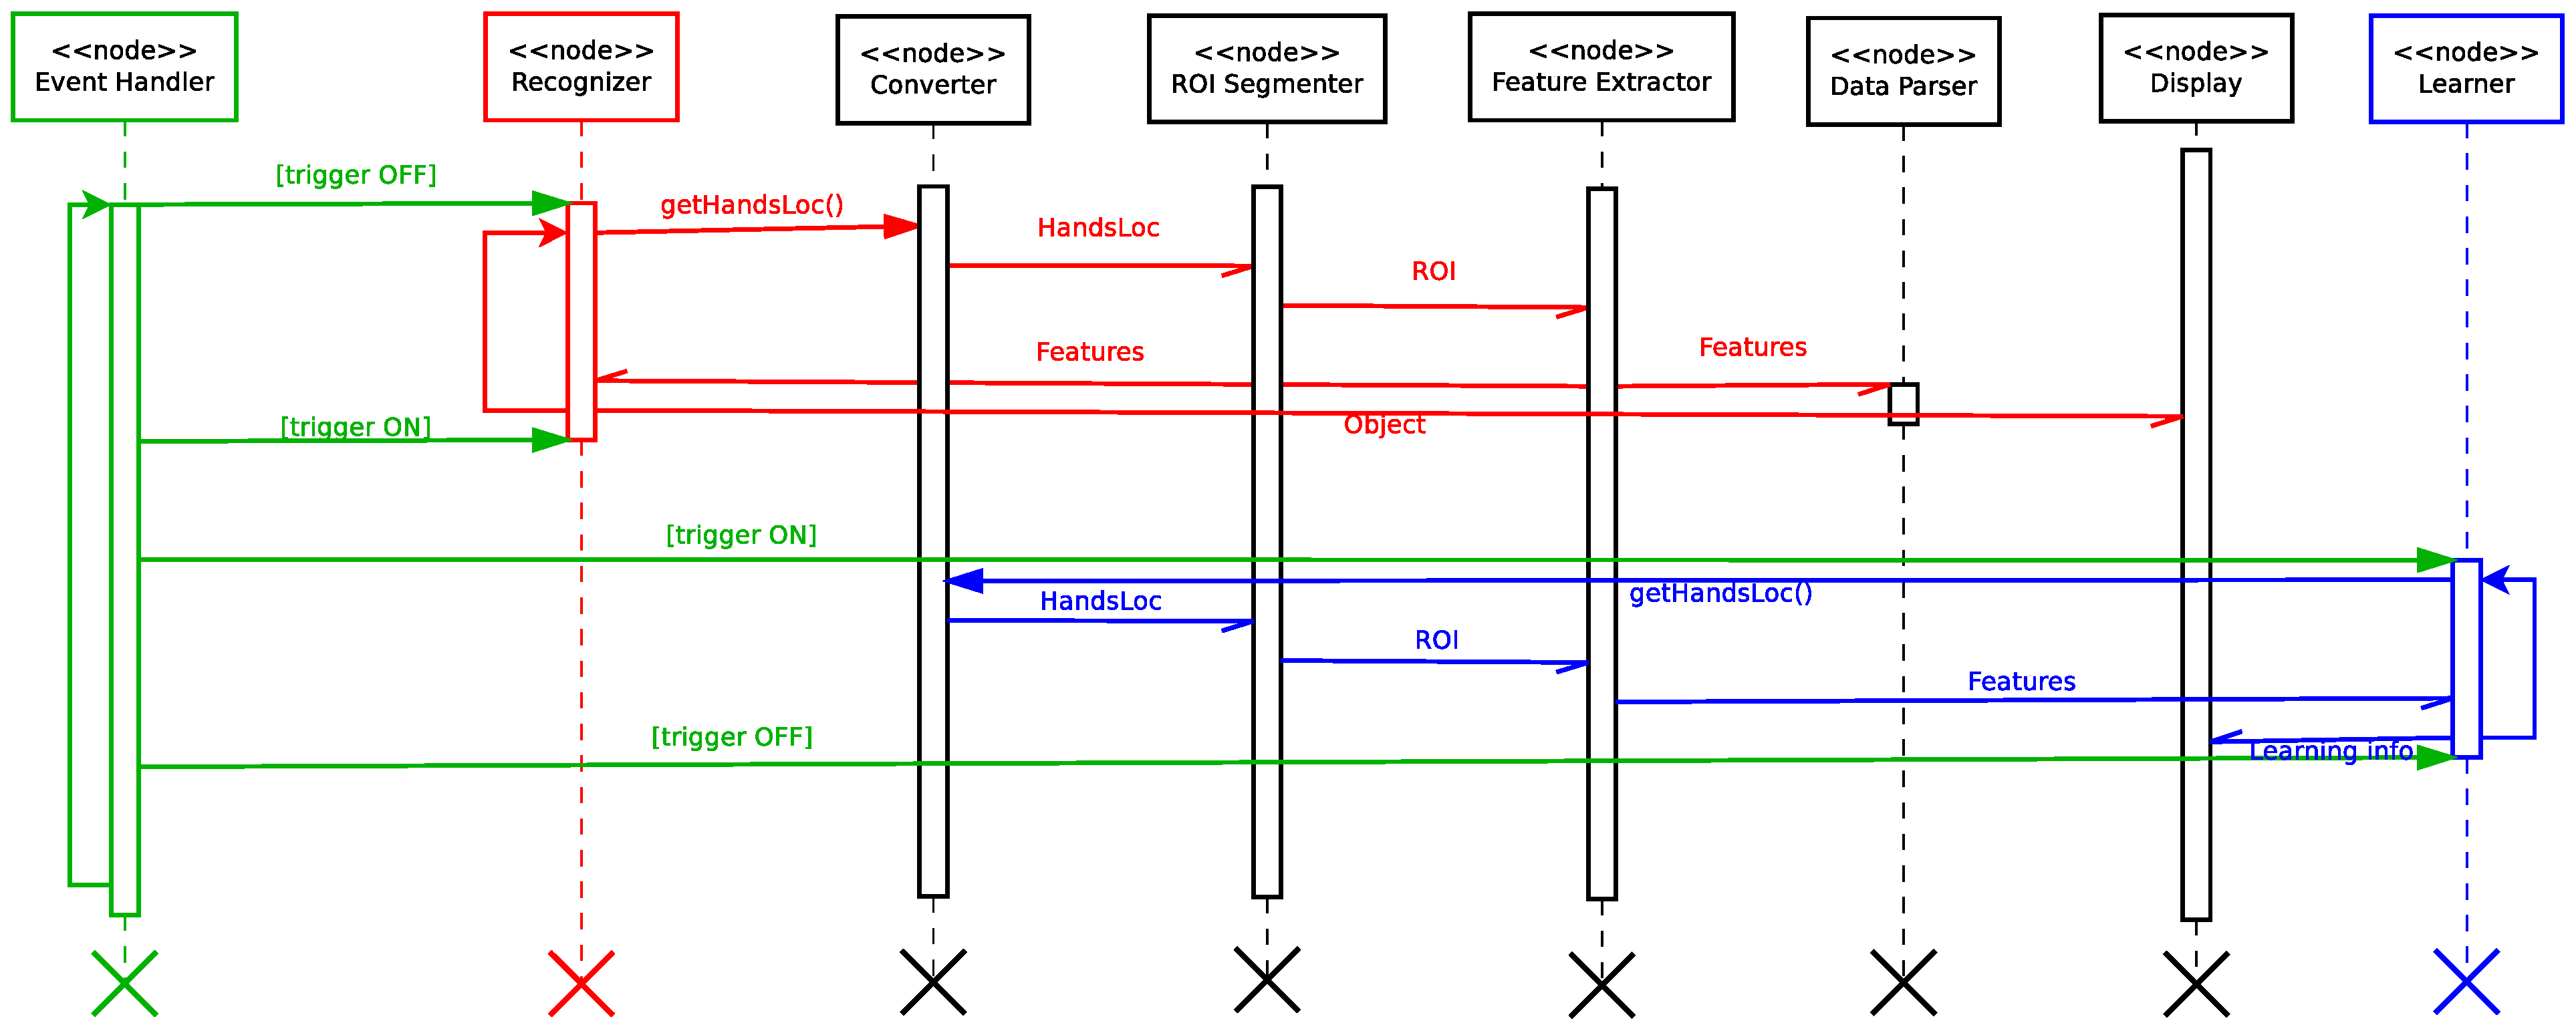
\includegraphics[scale=0.4]{../diagrams/images/sequence.eps}
\end{center}

\subsection{Flowchart}
In the following diagram, the flow of the program is represented. 
\begin{center}
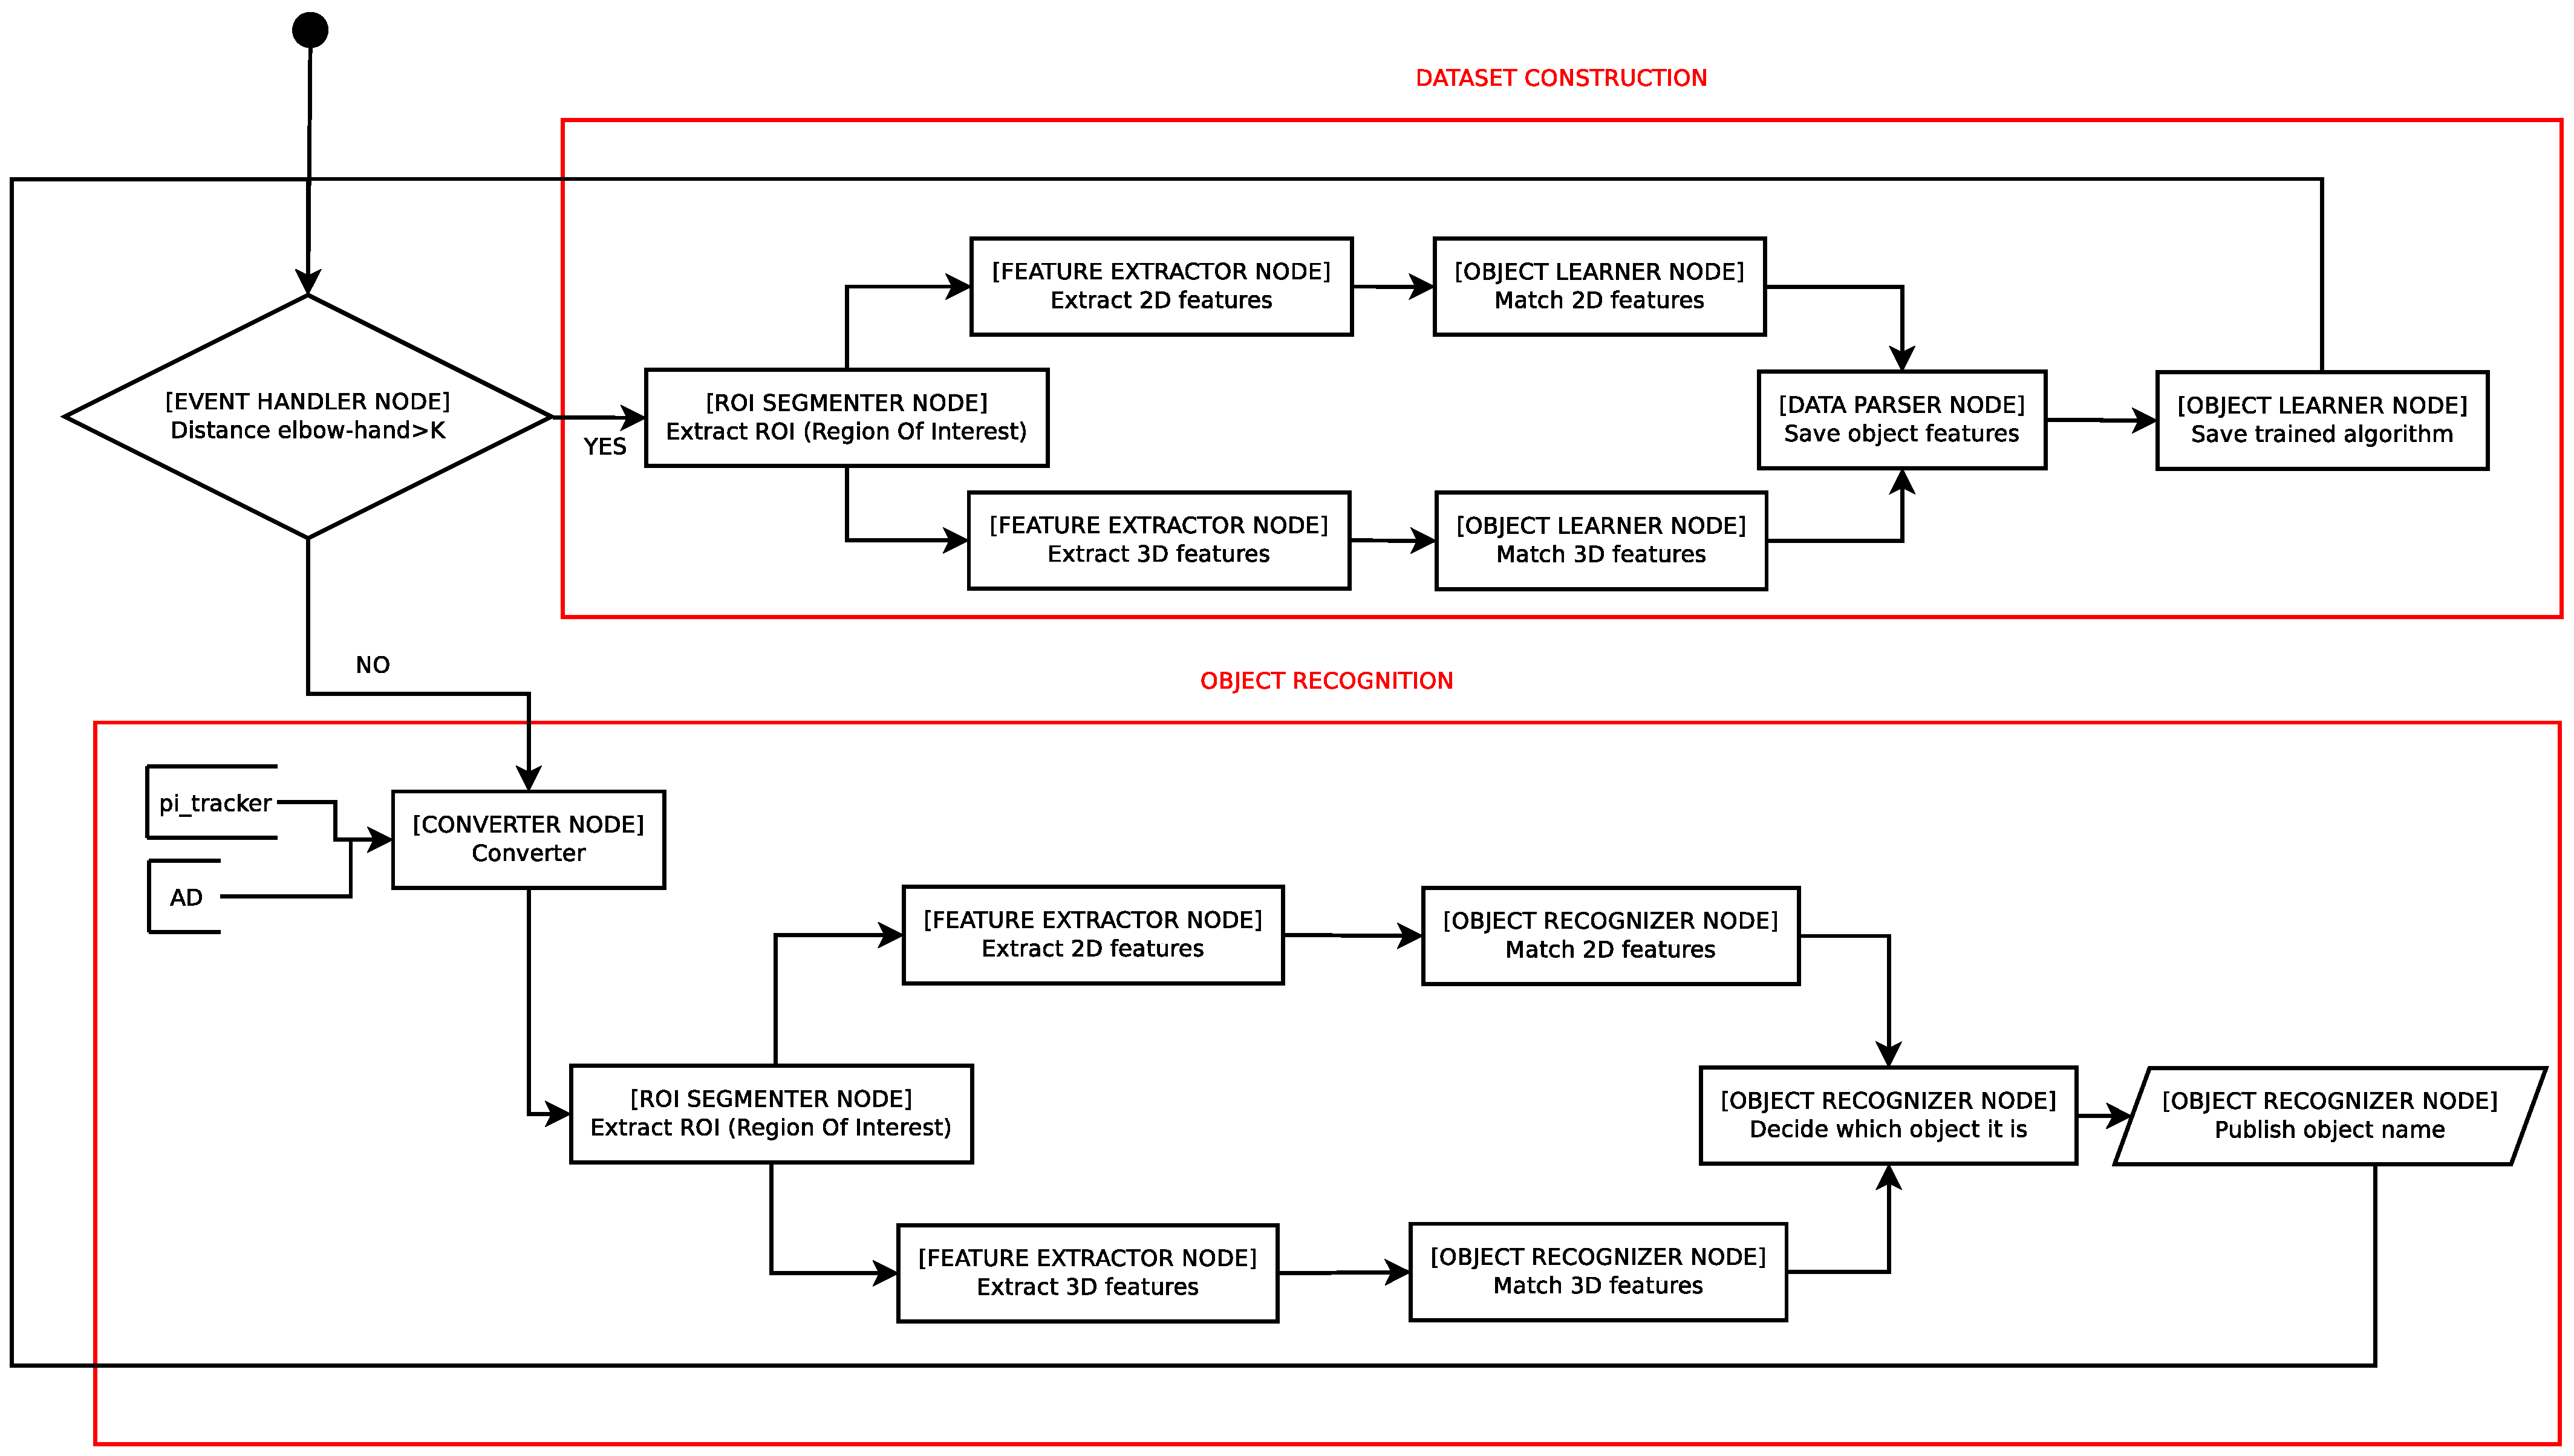
\includegraphics[scale=0.35]{../diagrams/images/flowcharts.eps}
\end{center}





\section{Functional requirements}

\subsection{General requirements}
\begin{enumerate}[label=\textbf{FR\threedigits*}, leftmargin=2cm]

	\item The software must be developed under ROS (Robotic Operating System), using the Groovy distro and rosbuild.
	\item A version control system should be used (GIT) and all the code must be periodically updated in the following github repository:  $https://github.com/irenesanznieto/TFG$
	\item The software has to have an interface. Its requirements are specified in the following "Interface Requirements" section. 
	\item The software must accept as inputs the following RGB-D sensors: Microsoft Kinect, ASUS Xtion PRO, ASUS Xtion PRO Live, PrimeSense PSDK 5.0.
	\item The output of the system must be a node specifying the name of the detected object. 
 
\subsection{Event Handler}
 
\subsection{Display}

\item The program must have one window with the output of the camera of the kinect sensor. 
\item The information as to what mode the program is in has to be shown in the title of the window.
\item In the recognition mode, the interface must show a square around the detected object and a text label indicating the object's name. Also, two points must be drawn in each of the hands. 
%\item The learning mode should open a new window where an shpere will appear. The sphere must show a different colour when a template of that zone is made. On the main window, a square should be placed around the new object. 
\item The learning mode should display the number of views obtained and processed of the object as well as an indication as to how to rotate the object to obtain further views. 


\subsection{Object Learner}
	\item The input to this node will be the features (both 2D and 3D) extracted from the feature extractor node. 
	\item This node must have two algorithms, one for 2D and other for 3D. 
	\item The algorithm used with 2D features should be a BruteForce trainer.
	\item The algorithm used with 3D features will be the Line-Mod trainer. 	
	\item This node must send feedback messages to the display with the learning information (number of views of the object processed, information about how to rotate the object).
	\item The output of this node will be the trained algorithms, whose parameters must be written to a file. 

\subsection{Object Recognizer}
	\item This node must have two algorithms, one for 2D and other for 3D. 
	\item The algorithm used with 2D features should be a BruteForce matcher.
	\item The algorithm used with 3D features will be the Line-Mod matcher. 
	\item A weighting must be made to the output of the matching process. This will help reduce the false positives and negatives by modelling occlusions depending on the hand-elbow relative positions. 
	\item A weighting must be made depending on the amount of texture possessed by each object to decide which matching should have more importance, the 2D or the 3D one. 



\subsection{Converter}

\item The information should be received subscribing to the topics of the different third-party packages. 
\item The internal message format must have the following structure: \\[0.3cm]
\textit{
std\_ msgs/Header header\\[0.1cm]
int32 id\\[0.1cm]
geometry\_ msgs/Vector3[] position\\
\hspace*{0.5cm}float64 x\\
\hspace*{0.5cm}float64 y\\
\hspace*{0.5cm}float64 z\\
}


\subsection{ROI Segmenter}
	\item This node will segment the Region Of Interest both in 2D (image) and in 3D (point cloud). 
	\item In the 3D segmentation, the ROI will be a box around the hand. 
	\item The original point cloud will be filtered using a depth filter to eliminate the background. After that, the dimensions of the box will be obtained locating the maximum and minimum points in the x, y and z axis. 
	\item The size of the 2D ROI must be extracted from the 3D ROI x and y dimensions. Those measures will be transformed to pixels. 
	\item The 2D ROI will be cropped from the original image using the points obtained from the 3D ROI. 

\subsection{Feature Extractor}
\item This node will extract both 3D and 2D features. 
\item The 2D features will be expressed as a vector of descriptors, using the ORB approach. 
\item The 3D features will be expressed as a vector of features, using the Line-Mod approach.

\item The 2D and 3D features of all the views of each object will be stored in a file, using the data parser node.  

\subsection{Data Parser}
\item This node will compress the features obtained to have one data file per object with all the information.
 
\item It has to be able to create a new file for storing the features of a new object. 
\item It has to be able to delete certain views or a complete file of the dataset. 
\item It has to be able to add another view to a previously stored object. 

\item This node will also be able to read the files to extract the 2D and 3D features of each object of the dataset. 

\item The name of the file will be the one given to the object. 

\item The datafile structure will be: \\
		\begin{lstlisting}
	<view1>
		<2D>
			[descriptor information ..]
		</2D>
		<3D>
			[template information ..]
		</3D>
	</view1>	
	...
	...
	...		
			
	<viewN>
		<2D>
			[descriptor information ..]
		</2D>
		<3D>
			[template information ..]
		</3D>
	</viewN>	
		
		\end{lstlisting}
	


\end{enumerate}





\section{Performance requirements}

\begin{enumerate}[label=\textbf{PR\threedigits*}]
\item The recognition must run on the lowest amount of time possible, to allow a fluid human-robot interaction. This time must be lower than 500 ms. 
\item The learning must run on the lowest amount of time possible, to allow a fluid human-robot interaction. This time must be lower than 5s. 
\end{enumerate}


%\section{Operational requirements}
%\section{Resource requirements}
%\section{Verification requirements}
%\section{Acceptance testing requirements}	%This is a validation activity; did we build the right thing? Is this what the customer really needs? 

\section{Documentation requirements}
\begin{enumerate}[label=\textbf{DR\threedigits*}]
	\item The code must be completely documented, i.e. each class, class function , class member and piece of code should have comments explaining all the aspects. 
	\item The documentation will be made using Doxygen notation, through the rosdoc\_ lite 
	% $[http://wiki.ros.org/rosdoc\_lite]$ 
	ROS package. 
	\item All the documentation must be available at the git repository. 
\end{enumerate}

%\section{Security requirements}
%\section{Portability requirements}
%\section{Quality requirements}
%\section{Reliability requirements}
\section{Maintainability requirements}
\begin{enumerate}[label=\textbf{MR\threedigits*}]
	\item The code must be as modular as possible. 
	\item All the classes' variables that are susceptible of being modified through a inheritance will be declared as protected. 
	\item Gtests will be built to demonstrate each functional requirement. 
	
\end{enumerate}

%\section{Safety requirements}

%\section{Time Schedule}


\end{document}



	\chapter{Project management}
	\label{project_management}
		 The present section describes the project management followed in this thesis. The Gantt diagram created for this purpose can be seen in the following page.
		 \\

		 The thesis was started on February 7th 2013 and was finished on July 11th 2014.    
		 The project management has suffered modifications throughout its development.  The final project management chart has three differentiated parts the learning phase, the project programming and the documentation phase. 
		 \begin{itemize}
			 	\item{\textbf{Learning phase}} \\
			 	This part consisted on a exploration of all the different technologies that could be used and the different state of the art techniques available. A thorough research on the object recognition and human tracking fields was performed. This research continued until the finishing of the thesis, but the most important part of it was made in this period of time. 
			 	\\

			 	The methods found were tested through demonstrations and there the main problems and possible solutions were obtained. This phase was crucial for the project, since in it the requisites of the software were defined as well as the technologies used and the general skeleton of the project's design that would later be implemented. 
			 	\\

			 	\item{\textbf{Project programming}}\\
			 	In this phase the project was coded and tested. The state of the art algorithms research continued to allow the overcoming of the different difficulties that appear when implementing theoretical concepts. This modified the project's design as well as some of the technologies applied in the thesis. 

			 	\item{\textbf{Documentation}}\\
			 	This final part of the project consisted on creating the documentation of the project and the present thesis. Also, the presentation documentation was prepared. 
			 	\\
		 \end{itemize}

		\begin{figure}[H]
			\centering
		    \includegraphics[scale=0.5, angle=90]{img/final.png}
			\caption[Gantt Diagram]{Gantt Diagram}	
			\label{gantt_diagram}
		\end{figure}

\newpage
	\chapter{Budget}
		This section presents the estimated budget of the project. 
		Section \ref{project_management} explained the time management followed in this project and the different phases it underwent. 
		Figure \ref{phases} shows the summary of the days spent in each of the phases. 
		The phase that occupied most of the time was the learning phase. 
		The state of the art learning occupies most of the project since it was performed in parallel with most of the other phases, as can be seen in figure \ref{gantt_diagram}. 
		The next phase in size is the project programming and then the documentation of the project. 
		% \begin{figure}[H]
		% 	\centering
		%     \includegraphics[width=0.8\linewidth]{img/budget/phases.png}
		% 	\caption[Days and hours per project phase]{Summary of the days and hours spent in each of the project's phases}	
		% 		    \label{phases}
		% \end{figure}


		\begin{table}[H]
\centering
\begin{tabular} {l c c c }
\toprule
\addlinespace[3mm]
   \multicolumn{1}{c}{\begin{center}\textbf{PHASE}\end{center}} &
   \multicolumn{1}{c}{\begin{center}\textbf{BEGIN DATE}\end{center}} &
   \multicolumn{1}{c}{\begin{center}\textbf{END DATE}\end{center}} &
   \multicolumn{1}{c}{\begin{center}\textbf{\hspace*{0.7cm}DAYS}\end{center}} &\\
\addlinespace[-3mm]
\midrule
Planning of the Thesis 	&	07/02/13 	&	25/02/13	&	18 \\	
State of the art	&	28/04/13	&11/07/14	&	439	\\
Learning 		&	26/02/13	&	29/10/13	&	185	** \\
\hspace*{0.5cm}	OpenCV	&	26/02/13 	&	24/04/13 	&	57	\\
\hspace*{0.5cm}	OpenCV Demo	&	25/04/13	&	25/04/13	&	MILESTONE	\\
\hspace*{0.5cm}	PCL + ROS	&	25/04/13	&	29/10/13	&	127	**		\\
\hspace*{0.5cm}	PCL + ROS Demo	&	30/10/13	&	30/10/13	&	MILESTONE	\\
Project Objectives Definition	&	30/10/13	&	07/11/13	&	8\\	
Design	&	08/11/13	&	21/11/13 	&	13	\\
Project Programming		&	22/11/13	&	20/05/14	&	179	\\
\hspace*{0.5cm}	pi\_tracker integration : converter &	22/11/13	&	20/01/14	&	59\\	
\hspace*{0.5cm}	ROI segmentation implementation		&	21/01/14	&	20/02/14	&	30	\\
\hspace*{0.5cm}	Feature extraction implementation	&	21/02/14	&	15/04/14	&	53\\	
\hspace*{0.5cm}	State machine implementation	&	16/04/14	&	14/05/14	&	28	\\
\hspace*{0.5cm}	Decision algorithm development	&	15/05/14	&	20/05/14	&	5	\\
\hspace*{0.5cm}	Tests	&	22/11/13	&	20/05/14	&	179\\	
Documentation	&	21/05/14	&	11/07/14	&	51	\\
\hspace*{0.5cm}		Thesis writing	&	21/05/14	&	22/06/14	&	32	\\
\hspace*{0.5cm}		Thesis hand-in	&	22/06/14	&	22/06/14	&	MILESTONE	\\
\hspace*{0.5cm}		Presentation preparation		&	23/06/14	&	11/07/14	&	18	\\
\hspace*{0.5cm}		Thesis presentation		&	11/07/14	&	11/07/14	&	MILESTONE	\\

\addlinespace[3mm]
\bottomrule
\addlinespace[3mm]

\textbf{TOTAL DAYS: 	}		&&&\textbf{	454}	\\
\textbf{TOTAL HOURS (3h per day) :} &&&			\textbf{1362}	\\
\addlinespace[3mm]

\bottomrule
\end{tabular}
\caption[Days and hours per project phase]{Summary of the days and hours spent in each of the project's phases.\\
** 60 days of holidays are not taken into account in the calculations.}	
\label{phases}

\end{table}



		It can be seen from figure \ref{phases} that the total days spent in the development of this project were 454. 
		It was assumed that around 60 days between the begin and end dates were not devoted to this thesis. 
		Also, an average of 3 hours per day were reserved to implementing this system and hence the total hours used were 1362. 
		The man hours performed by my advisor were calculated as one hour per week as average. 
		Figure \ref{budget} shows the final budget of the project. 
		The first two items are the hardware required, then the man hours cost and finally the software cost. 
		It can be noted that the software total cost was of 0 \euro. 
		This is because all software used in this system is Open Source, hence no licenses are paid. 


		% \begin{figure}[H]
		% 	\centering
		%     \includegraphics[width=0.8\linewidth]{img/budget/budget.png}
		% 	\caption[Project's budget]{Project's budget}	
		%     \label{budget}
		% \end{figure}

\begin{table}[H]
\centering
\begin{tabular} {l c c c c}
\toprule
\addlinespace[3mm]
   \multicolumn{1}{c}{\begin{center}\textbf{ITEM}\end{center}} &
   \multicolumn{1}{c}{\begin{center}\textbf{COST (\euro)}\end{center}} &
   \multicolumn{1}{c}{\begin{center}\textbf{UNITS}\end{center}} &
   \multicolumn{1}{c}{\begin{center}\textbf{QUANTITY}\end{center}} &
   \multicolumn{1}{c}{\begin{center}\textbf{TOTAL COST (\euro)}\end{center}} &
\\
\addlinespace[-3mm]
\midrule
\textbf{Hardware}	&&&&		\\					
\hspace*{0.5cm}	Kinect 360	&	120	&	\euro/unit	&	1 	&	120 \\
\hspace*{0.5cm}	Mountain Ivy 11 Laptop	&	1000	&	\euro/unit	&	1	&	1000\\		
\textbf{Man hours}													&&&&		\\		
\hspace*{0.5cm}	Senior Engineer 	&	12	&\euro/h	&	56.75	&	681\\
\hspace*{0.5cm}	Undegraduate Engineer	&	8	&	\euro/h		&	1362	&	10896 \\
						
\textbf{Software}			&&&&		\\						
						
\hspace*{0.5cm}	Linux	&	0 &	\euro/license	&	1	&	0\\
\hspace*{0.5cm}	ROS	&	0	&\euro/license&	1	&0\\
\hspace*{0.8cm}		openni\_camera	&	0	&	\euro/license	&1&		0\\
\hspace*{0.8cm}		openni\_launch	&	0	&	\euro/license	&1&	0\\
\hspace*{0.8cm}		pi\_tracker 		&	0	&	\euro/license	&1&	0\\
\hspace*{0.5cm}	PCL		&	0	&	\euro/license	&	1	&	0\\
\hspace*{0.5cm}	OpenCV	&	0	&	\euro/license	&	1	&	0\\
						
\midrule

\textbf{TOTAL PROJECT'S COST: }			&&&&			\textbf{12697}\\

\bottomrule
\end{tabular}
\caption[Project's budget]{Project's budget}
\label{budget}

\end{table}


		Since all the software used is Open Source, I have performed an estimation of the cost of the development of each of the libraries I have used in this project. 
		Figure \ref{estimations} summarizes the results.  

		% \begin{figure}[H]
		% 	\centering
		%     \includegraphics[width=0.6\linewidth]{img/budget/estimations.png}
		% 	\caption[Open source software cost estimation]{Open source software cost estimation}
		%     \label{estimations}	
		% \end{figure}





\begin{table}[H]
\centering
\begin{tabular} {l c}
\toprule
\addlinespace[3mm]
   \multicolumn{1}{c}{\begin{center}\textbf{SOFTWARE}\end{center}} &
   \multicolumn{1}{c}{\begin{center}\textbf{TOTAL COST (\euro)}\end{center}} &
\\
\addlinespace[-3mm]
\midrule
Linux	&	10680392	\\
ROS		&	2932343.25	\\
\hspace*{0.5cm}	openni\_camera	&	99315.98	\\
\hspace*{0.5cm}	openni\_launch	&	5956.98		\\
\hspace*{0.5cm}	pi\_tracker 	&	74092.69	\\
PCL	&	13101526.72		\\
OpenCV	&	36263862.04		\\
OCULAR	&	58709.439	\\

\bottomrule
\end{tabular}
\caption[Open source software cost estimation]{Open source software cost estimation}
\label{estimations}

\end{table}


		The estimations are created using the SLOCCount Open Source program \cite{sloccount}. 
		This software measures the number of lines and automatically estimates the effort, time and money needed to create the software. 
		The figures in table \ref{estimations} are obtained using the basic COCOMO model. 
		All defaults were used and the final cost of developing each of the tools are the ones presented in figure \ref{estimations}. 
		It is important to note that in the case that these projects were not Open Source the cost of using them would not be, of course, the cost of the complete development. 
		Instead, the right to use of the software is usually given in exchange of the payment of a license. 
		\\

		The cost estimation of the system developed in this thesis was also performed. 
		It can be seen the high difference between the real cost and the estimated one. 
		This is mainly due to the difference in the man-hours cost. 
		By default, the software assumes a yearly cost per man of around 56 k USD which means an hourly rate of around 20 USD per hour, or 15 \euro. 
		The final cost of the developed thesis is less than 13000 \euro, including all the required hardware. 

\end{appendices}